\documentclass{article}
\usepackage[margin=1in]{geometry}
\usepackage{amsmath,amsthm,amssymb}
\usepackage{bbm,enumerate,mathtools}
\usepackage{tikz,pgfplots}
\usepackage{chessboard}
\usepackage[hidelinks]{hyperref}
\usepackage{multicol} % Problem 35
\usepackage{xstring} % Difficulty command
\usetikzlibrary{shapes.geometric}

\newenvironment{question}{\begin{trivlist}\item[\textbf{Question.}]}{\end{trivlist}}
\newenvironment{note}{\begin{trivlist}\item[\textbf{Note.}]}{\end{trivlist}}
\newenvironment{references}{\begin{trivlist}\item[\textbf{References.}]}{\end{trivlist}}
\newenvironment{related}{\begin{trivlist}\item[\textbf{Related.}]\end{trivlist}\begin{enumerate}}{\end{enumerate}}

\newcommand\score[1]{
\pgfmathsetmacro\pgfxa{#1+1}
\tikzstyle{scorestars}=[
  star,
  star points=5,
  star point ratio=2.25,
  draw,
  inner sep=3pt,
  anchor=outer point 5
]
  \begin{tikzpicture}[baseline]
    \draw[opacity=0] (0,-0.5) rectangle (0,0.2); % Workaround for whitespace at the bottom.
    \foreach \i in {1,...,4} {
      \pgfmathparse{(\i<=#1?"yellow":"gray")}
      \edef\starcolor{\pgfmathresult}
      \draw (\i*4.5ex,0) node[name=star\i,scorestars,fill=\starcolor]  {};
    }
  \end{tikzpicture}
}

\newcommand{\difficulty}[1]{%
  \IfEqCase{#1}{%
      {1}{
        
\begin{tikzpicture}[scale=0.7, baseline=0.9mm]%
          \definecolor{slopegreen}{rgb}{0.0, 0.5, 0.0}%
          \fill[slopegreen] (0.5,0.5) circle (0.5);%
        \end{tikzpicture}%
      }%
      {2}{
        
\begin{tikzpicture}[scale=0.7, baseline=0.9mm]%
          \definecolor{slopeblue}{rgb}{0.0, 0.44, 1.00}
          \fill[slopeblue] (0,0) rectangle (1,1);%
        \end{tikzpicture}%
      }%
      {3}{
\begin{tikzpicture}[scale=0.7, baseline=0.9mm]\fill (0,0.5)--(0.5, 0)--(1,0.5)--(0.5,1)--cycle; \end{tikzpicture}}%
      {4}{
\begin{tikzpicture}[scale=0.7, baseline=0.9mm]\fill (0.25,0)--(0,0.5)--(0.25,1)--(0.5,0.5)--cycle; \fill (0.75,0)--(0.5,0.5)--(0.75,1)--(1,0.5)--cycle;\end{tikzpicture}}%
      % you can add more cases here as desired
  }[\PackageError{difficulty}{Undefined difficulty level: #1}{}]%
}%
\newcommand{\rating}[2]{\difficulty{#1}\\\score{#2}\\}


\begin{document}
\rating{2}{2}
Euler's well is a labeling of the $n \times k$ grid with a permutation in
$S_{n \times k}$ such that the upper left corner is labeled with $1$.
\begin{quote}
  Water is poured into the well from a point above the section marked 1, at the rate of 1 cubic foot per minute. Assume that water entering a region of constant depth immediately disperses to all orthogonally adjacent lower-depth regions evenly along that region’s exposed perimeter (an assumption that Euler insisted on).

After how many minutes will the water begin to accumulate in
[the lower right corner]?
\end{quote}

\begin{figure}[ht!]
  \centering
  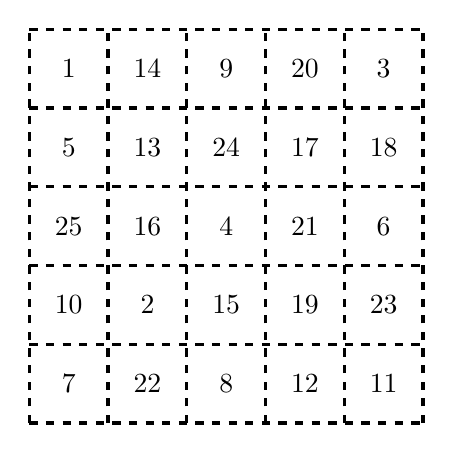
\begin{tikzpicture}
    \draw[dashed, very thick] (0,0) grid (5,5);
    \foreach \i/\j/\n in {
      0/4/1, 1/4/14, 2/4/9, 3/4/20, 4/4/3,
      0/3/5, 1/3/13, 2/3/24, 3/3/17, 4/3/18,
      0/2/25, 1/2/16, 2/2/4, 3/2/21, 4/2/6,
      0/1/10, 1/1/2, 2/1/15, 3/1/19, 4/1/23,
      0/0/7, 1/0/22, 2/0/8, 3/0/12, 4/0/11,} {
      \node at (\i + 0.5, \j + 0.5) {\n};
    }
  \end{tikzpicture}
  \caption{
    A labeling of the $5 \times 5$ grid where the labels are a permutation of
    the integers from $1$ to $25$.
  }
\end{figure}
\begin{question}
  For a random permtation in $S_{n \times k}$, what is the expected amount of
  time it takes for water to reach the lower right hand corner of the grid?
\end{question}

\begin{related}
  \item What if water can flow diagonally?
  \item What if the source or sink are in different places? What if there are
  multiple sources/sinks?
  \item What if this is done on a torus? Triangular/hexagonal grid? Three
  dimensions?
  \item What if the numbers are not neccesarily a permutation?
  \item What if the well is a Latin square?
  \item What is an efficient algorithm for computing this for an arbitrary
  permutation?
  \item What is the expected value of number of ``wet'' squares at the end?
  \item How many wells have minimal filling times?
  \item How many wells up to ``fill level''? (e.g. two wells are equivalent if
  each square has the same height after the water flows all the way)
\end{related}

\begin{references}
  \item \url{http://chalkdustmagazine.com/blog/well-well-well/}
  \item \url{https://oeis.org/A321853}
\end{references}

\end{document}
